% 2007 年山东卷理科第 19 题：直四棱柱 ABCD-A1B1C1D1。
%   底面 ABCD 为直角梯形：AD⊥DC，AB∥DC，DC=DD1=2AD=2AB。
%   E 为 DC 中点。图中画出 A1B、BD、C1B、C1D、D1E 等辅助线。
% 来源 PDF：gaokaomath-src/普通高考/2007/2007山东理.pdf
% SHA-256：4388fb6a3d728a0f289c751eba4ea096b5b256ed446bbec3d60c3240f53d7864
% 原页：2007山东理.pdf 第 2 页（A3 三栏）第 1 栏，书页码 398。
% 重绘依据：斜投影，D(0,0)、C(2.2,0)，纵深向量 (0.55,0.75) 对应 AD=1，
%   AB=1 沿 DC 方向，DD1=2 竖直向上；被遮棱 DA、AB、AA1 画虚线。
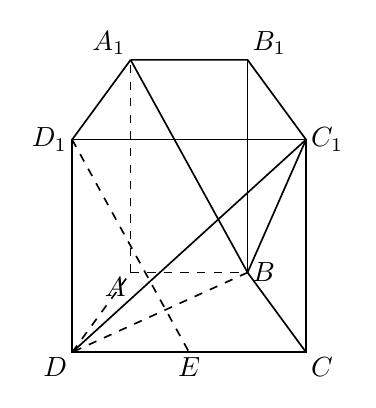
\begin{tikzpicture}[scale=1.35, semithick,
  every node/.style={inner sep=1.5pt}]
  \coordinate (D)  at (0,0);
  \coordinate (C)  at (2.2,0);
  \coordinate (A)  at (0.55,0.75);
  \coordinate (B)  at (1.65,0.75);
  \coordinate (D1) at (0,2.0);
  \coordinate (C1) at (2.2,2.0);
  \coordinate (A1) at (0.55,2.75);
  \coordinate (B1) at (1.65,2.75);
  \coordinate (E)  at (1.1,0);

  % 被遮棱
  \draw[dashed] (D) -- (A);
  \draw[dashed] (A) -- (B);
  \draw[dashed] (A) -- (A1);
  % 辅助线
  \draw[dashed] (B) -- (D);
  \draw[dashed] (D1) -- (E);
  \draw (A1) -- (B);
  \draw (C1) -- (B);
  \draw (C1) -- (D);
  % 可见棱
  \draw (D) -- (C) -- (C1) -- (D1) -- cycle;
  \draw (D) -- (D1);
  \draw (C) -- (C1);
  \draw (A1) -- (B1) -- (C1);
  \draw (A1) -- (D1);
  \draw (B1) -- (B);
  \draw (B) -- (C);

  % 顶点标注
  \node[below left]  at (D)  {$D$};
  \node[below right] at (C)  {$C$};
  \node[below left]  at (A)  {$A$};
  \node[right]       at (B)  {$B$};
  \node[left]        at (D1) {$D_1$};
  \node[right]       at (C1) {$C_1$};
  \node[above left]  at (A1) {$A_1$};
  \node[above right] at (B1) {$B_1$};
  \node[below]       at (E)  {$E$};
\end{tikzpicture}
